\chapter{Goal Oriented Action Planning}

Das Goal Oriented Action Planning Planung Entscheidungssystem ist zur Planung zu einem bestimmten Ziel gedacht. Planung ist der Prozess der Suche einer Sequenz an Aktionen zur Erreichung eines Zieles. Die Suche kann dabei als Suchproblem dargestellt werden. Für das Verständnis wird daher Kenntnis der Themen Suchalgorithmen und Suchprobleme benötigt.



\section{Historie}

Das Entscheidungssystem \textit{Goal Oriented Action Planning} (\textit{GOAP}) entstand in der Entwicklung des Videospiel \textit{F.E.A.R First Encounter Assault Recon (2005)}. Die Entwickler wollten ein Videospiel entwickeln, das wie ein Actionfilm wirkt, mit intensiven Kämpfen. Für die intensiven Kämpfe benötigt man NPC, welche Deckung nehmen, blind feuern, über Fenster springen, Granaten werfen, untereinander kommunizieren und weitere Aktionen ausführen können.

Zuvor nutzte \textit{Monolith} Finite State Machines (\textit{FSM}) als Entscheidungssystem. Den Entwicklern fiel es jedoch zunehmend aufwendig, eine FSM mit neuen Zuständen und den dazugehörigen Aktionen zu erweitern. In einem vorherigen Videospiel \textit{No One Lives Forever (2000)}, wurde veruscht eine dynamische FSM zu implementieren, die sich an Zielzustände anpassen konnte. Allerdings wurde auch diese Lösung als zu unflexibel wahrgenommen. Aus dem Versuch der dynamischen FSM und STRIPS hat Jeff Orkin das GOAP System entwickelt, welches Echtzeitplanung erfüllen soll. Eine der Herausforderungen, mit denen sich Jeff Orkin während der Entwicklung konfrontiert sah, war die Berücksichtigung der Performance.\autocite{retro_fear}



\section{GOAP Bestandteile}

Das GOAP -System basiert dabei auf dem STRIPS System. Wie auch STRIPS besitzt GOAP Ziele, welche einen gewünschten Zustand beschreiben und Aktionen mit Effekten die Zustände ändern können. GOAP sucht nach einer Sequenz an Aktionen die das Ziel des NPC erreichen kann. Im Sinne von Jeff Orkins geschieht die eigentliche Ausführung der Aktionen über eine Finite State Machine (\textit{FSM}).


\subsection{Finite State Machine in GOAP}

Eine FSM wurde im Videospiel \textit{F.E.A.R} für die Ausführung der Aktionen benötigt. Die NPC führten ihre Aktionen durch eine Kombination aus Animationen und Bewegungen aus. Beispielsweise sorgte eine Cover-Aktion dafür, dass der NPC hinter eine Deckung lief und dort eine Deckungs-Animation abspielte. Eine Shoot-Aktion hingegen aktivierte eine entsprechende Schuss-Animation.
Die FSM bestand dabei aus den drei Zuständen GoTo, Animate und UseSmartObject. 

\begin{figure}[h]
  \centering
  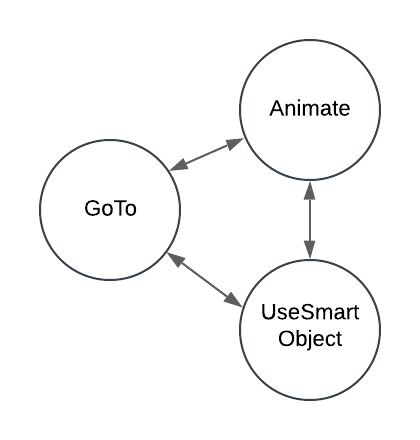
\includegraphics[width=7cm]{GOAP/GOAP_FSM}
	\captionsetup{justification=justified, format=plain}
  \caption{GOAP Finite State Machine}
  \label{GOAP_FSM}
\end{figure}

\textit{Monolith} hat durch die Zustände Animate und UseSmartObject Animationen umgesetzt.
von \textit{Monolith}


\subsection{GOAP Ziele}

Ein Ziel $GOAL(g)$ in GOAP setzt die erwünschte Zielzustände für den Planer. So setzt das Ziel $EliminatePlayer$ den Zielzustand $\{\lnot PlayerAlive\}$. 
\begin{align*}
GOAL(EliminatePlayer) = \{\lnot PlayerAlive\}
\end{align*}
Die Auswahl des Zieles geschieht nach ihrer Priorität und ob dieses gültig ist. Das Ziel mit der höchsten Priorität und Gültigkeit wird bevorzugt. Die Gültigkeit und Priorität basiert dabei auf dem Zustand $s$ des NPC und seiner Umwelt.
\begin{align*}
s = \{\lnot PlayerVisible\} \\
PRIORITY(s,EliminatePlayer) = 100 \\
VALID(s,EliminatePlayer) = false
\end{align*}


\subsection{GOAP Aktionen}

Aktionen können Weltzustände oder auch direkte Zustände eines NPC ändern. So kann beispielsweise die Aktion \textit{Reload} den Zustand $s = \{\lnot GunLoaded\}$ ändern.
\begin{align*}
TRANSITIONS(s,Reload) &= \{GunLoaded\}
\end{align*}
Dadurch haben Aktionen die Möglichkeit Zielzustände zu erreichen. Nehmen wir an der NPC hat das Ziel $Patrol$ und die Aktion $GoPatrol$ mit $TRANSITIONS(s,GoPatrol) = {AtPatrol}$, dann kann diese Aktion den Zielzustand erreichen.
Eine Aktion hat auch Vorbedingungen als Zustände, diese Zustände können wiederum von anderen Aktionen erfüllt werden. So könnte beispielsweise die Aktion $Reload$ die Vorbedingung der Aktion $Shoot$ erreichen.
\begin{align*}
PRECONDITION(Shoot) = \{GunLoaded\}
\end{align*}
Eine Aktion setzt auch wie im Suchproblem eine $ACTIONCOST$ Funktion um, die später zur Auswahl einer Aktion herangezogen wird. Wird die Aktion ausgewählt wird diese später von der FSM ausgeführt.


\subsection{Fallbeispiel}

Nehmen wir an, dass der NPC den Ausgangszustand $s$ besitzt und das Ziel $EliminatePlayer$.
\begin{align*}
s = \{PlayerVisible, \lnot GunLoaded\} \\
GOAL(EliminatePlayer) = \{\lnot PlayerAlive\}
\end{align*}
Der NPC muss nun versuchen das Ziel mit den möglichen Aktionen den Zielzustand $\{\lnot PlayerAlive\}$ erreichen. Die möglichen Aktionen werden dabei aus einer $ACTIONS(s)$ Funktion gelesen.
\begin{align*}
ACTIONS(s) = \{Reload, MoveToCover\} \\
TRANSITIONS(s,Reload) = \{GunLoaded\} \\
TRANSITIONS(s,MoveToCover) = \{AtCover\}
\end{align*}
Aus den $TRANSITIONS$ Funktion können wir entnehmen, dass keine der Aktionen den Zustand $\lnot PlayerAlive$ direkt erreichen kann. Außerdem müssen wir beachten, dass nicht jede Aktion auch das Ziel erreichen kann. Die Auswahl der Aktion geschieht durch den A* -Algorithmus.



\section{Unterschiede STRIPS und GOAP}

Die Hauptunterschiede von STRIPS und GOAP befinden sich dabei bei den eigentlichen Aktionen. Aktionen in GOAP haben Kosten und statt einer Add und Delete List ein Array an Preconditions und Effekten, die den World State verändern.

Aktionen in STRIPS haben im Gegensatz zu GOAP keine Kosten. Anhand der Kosten kann der GOAP Aktionen über andere Aktionen bestimmen. So sollen Aktionen mit geringeren Kosten bevorzugt werden.

STRIPS realisiert Effekte einer Aktion über eine Add und Delete List. Die Delete List löscht Wissen über Zustände. Während die Add List neues Wissen Zustände hinzufügt. In GOAP haben Aktionen Arrays die Preconditions und Effekte speichern. Procedural Preconditions Checks sorgen in GOAP dabei, dass nur Effekte genutzt werden, die erfüllte Preconditions haben. Die Effekte der GOAP Aktionen werden auch nicht direkt umgesetzt. Die Aktionen besitzen eine Funktion, die die Aktion ausführt. Während der Ausführung der Aktion können sich dabei die gewünschten Zustände ändern.